\documentclass[12pt]{article}
\usepackage[scaled]{helvet}
\renewcommand\familydefault{\sfdefault} 
\usepackage[T1]{fontenc}

\usepackage[english]{babel}
\usepackage[utf8]{inputenc}
\usepackage{amsmath}
\usepackage{bm}
\usepackage{parskip}
\usepackage{hyperref}
\usepackage{graphicx}
\usepackage{listings}
\usepackage{xcolor}

\definecolor{Brown}{cmyk}{0,0.81,1,0.60}
\definecolor{OliveGreen}{cmyk}{0.64,0,0.95,0.40}
\definecolor{CadetBlue}{cmyk}{0.62,0.57,0.23,0}
\definecolor{lightlightgray}{gray}{0.9}

\lstset { %
    language=C++,
    %backgroundcolor=\color{black!5}, % set backgroundcolor
    %basicstyle=\footnotesize,% basic font setting
	basicstyle=\ttfamily,                   % Code font, Examples: \footnotesize, \ttfamily
	keywordstyle=\color{OliveGreen},        % Keywords font ('*' = uppercase)
	commentstyle=\color{gray},              % Comments font
	backgroundcolor=\color{lightlightgray},
	tabsize=4,
	frame=single,
}

\title{\textbf{Practical 7: Rigid Bodies, part 2 }}
\author{Babis Koniaris}
\date{}

\begin{document}
\maketitle

\begin{center}
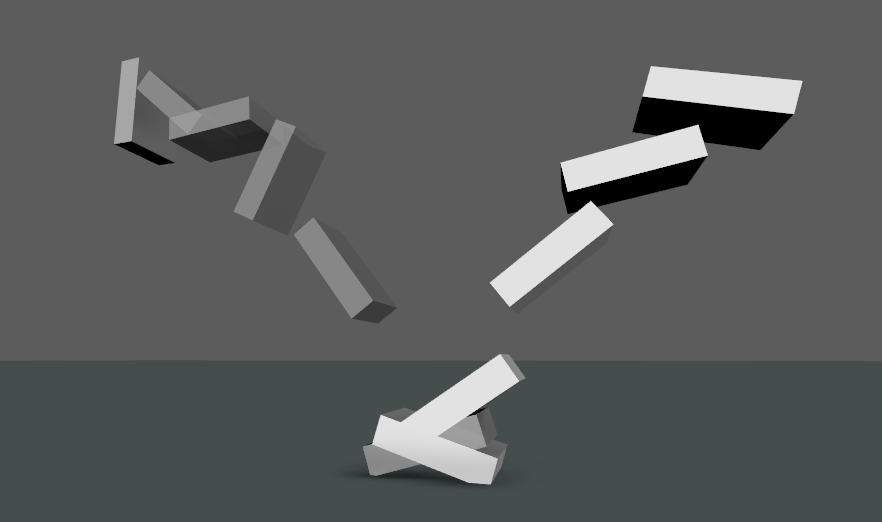
\includegraphics[width=\textwidth]{p7-teaser.png}
\end{center}
\pagebreak

\section*{Introduction}

The goals of this practical are to:

\begin{itemize}
\item Assign and maintain correct inertia tensors for cuboids
\item Apply impulses to rigid bodies
\item Apply correct bounce impulse to rigid body colliding with a plane
\end{itemize}

\section*{Tasks}

\subsection*{Task 1: Inertia tensor}

As we’ve seen in the lecture, the inertia tensor is to torque what mass is to acceleration. Unfortunately, it is not as simple to work with as mass is. Not only is it a matrix rather than a scalar, it depends on the geometry of the solid, and it also depends on its orientation. Computing the inertia tensor of a random solid model isn’t trivial, but luckily, the inertia tensors for common primitives are simple and well-documented. Please refer to the following page reference: \url{https://en.wikipedia.org/wiki/List_of_moments_of_inertia}. Since we are working with cuboids for the time being, here’s the inertia tensor of a cuboid of width $w$ (along the $x$ axis), height $h$ (along the $y$ axis), depth $d$ (along the $z$ axis) and mass $m$:

\begin{align}
I_0 = \begin{bmatrix}
\frac{1}{12}m(h^2+d^2) & 0 & 0\\ 
0 & \frac{1}{12}m(w^2+d^2) & 0\\ 
0 & 0 & \frac{1}{12}m(w^2+h^2)\\ 
\end{bmatrix}
\end{align}

\textbf{Task 1: \emph{Create} and \emph{maintain} a correct inverse inertia tensor for a cuboid}

You will have noticed that there are two parts to this task: creating and maintaining. Also notice that we will not store the tensor, but its inverse, as it is what we need in our simulation. Creating a valid tensor is easy, you can do so using the above formula. However, it must be updated any time the mass and dimension of the solids are modified. There are two design options to consider to achieve this: 

\begin{itemize}
\item Calculate the tensor dynamically. In other words, you don’t need to store the inverse tensor in a variable like m\_invInertia, instead the accessor method InverseInertia() computes the matrix any time it is called. The benefit of this approach is that this single method ensures that the inertia is always correct without having to modify any other part of our code. The drawback is cost: InverseInertia() will get called at every step of the simulation, so this would be unwelcome computation. 
\item Make sure the tensor (or in our case inverse tensor) is updated whenever the mass or dimensions of the body are updated. This approach requires the modification of more code, but it is computationally cheaper. This is the one I recommend that you implement. 
\end{itemize}

Also remember that the inertia (and inverse inertia) also depend on the orientation (i.e., rotation matrix) of the rigid body:

\begin{align}
I(t) = R(t)I_0R(t)^T \\
I^{-1}(t) = R(t)I_0^{-1}R(t)^T
\end{align}

\subsection*{Task 2: Applying impulses}

The goal of this task is to allow you to understand the effect of applying impulses at various points on a solid. In what follows, you will work with a cuboid named rb that has a mass $m = 1$ and the following dimensions:
\begin{itemize}
\item width = 2
\item height = 6
\item depth = 2
\end{itemize}
This corresponds to a default cubic rigid body that has been scaled by a vector (1,3,1).

\textbf{Task 2: Experiment with the application of impulses to a rigid body}

Here are examples of tests you should carry out:
\begin{itemize}
\item Give rb an initial velocity of (0,0,0) and an angular velocity of (0,0,0). In other words, rb is immobile! No force applies to rb. After 2 seconds:
	\begin{itemize}
	\item Apply an impulse that will make rb move to the left with a velocity of (-1,0,0)
	\item Apply an impulse that will make rb move to the left with a velocity of (-1,0,0) and start spinning anticlockwise around the z axis
	\end{itemize}
\item Give rb an initial velocity of (3,0,0) and an angular velocity of (0,0,0). No force applies to rb. After 2 seconds:
	\begin{itemize}
	\item Apply an impulse that will make rb stop moving
	\item Apply an impulse that will make rb change direction and travel with a velocity of (-3,0,0).
	\item Apply an impulse that will make rb stop translating and start spinning clockwise
	\end{itemize}
\item Consider that rb is traveling with a constant velocity of (3,0,0) and angular velocity of (0,0,1). No force applies to rb. After 2 seconds:
	\begin{itemize}
	\item Apply an impulse that will make rb stop moving and rotating
	\end{itemize}
\end{itemize}

\subsection*{Task 3: Collision response}

\textbf{Task 3: Simulate the collision between a rigid body (cuboid) and a fixed horizontal plane using impulse-based collision response.}

Collision response can be managed in different ways. We are going to implement an impulse-based response in which some coarse approximations will be made. The work involves these two parts:

\begin{itemize}
\item Once you have detected that a component (vertex, edge or face) overlaps with the ground plane, translate the body up so that the component lies exactly on the ground. This is a rough way of managing collisions, but it is simple to implement and should work reasonably well.
\item Apply the correct collision impulse at the correct point on the rigid body (as described in the lecture).
\end{itemize}

\subsection{Further tasks}

Collisions without friction look very unnatural: a solid that falls down on the ground will always bounce along the same vertical axis, regardless of the way it hits the ground. To make the bounces look more believable, friction must be simulated. Try to come up with a friction model that make bounces look more believable if you have time. You will learn how friction can be simulated next week... 

%\section*{Deliverables}

%Nothing has to be handed in this week but the work you have completed will be a part of the assessed deliverables of next week’s practical. Make sure you complete this assignment this week or you will run out of time if you try to do everything next week.

\end{document}